% *********************************************************************
% © 2016–2026 Jeremy Sylvestre
%
% Permission is granted to copy, distribute and/or modify this document
% under the terms of the GNU Free Documentation License, Version 1.3 or
% any later version published by the Free Software Foundation; with no
% Invariant Sections, no Front-Cover Texts, and no Back-Cover Texts. A
% copy of the license is included in the appendix entitled “GNU Free
% Documentation License” that appears in the output document of this
% PreTeXt source code. All trademarks™ are the registered® marks of
% their respective owners.
%
% *********************************************************************
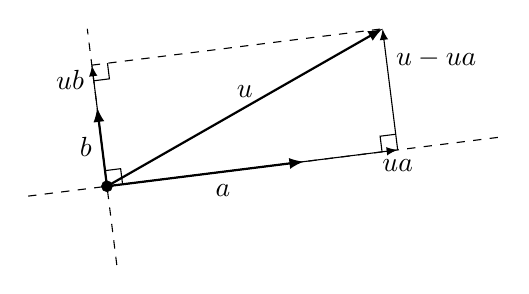
\begin{tikzpicture}[
	point/.style={circle,draw,very thin,fill,inner sep=0pt,minimum size=4pt},
	vector/.style={-latex},
]
	\coordinate (o) at (0,0);
	% line slope 1/8, perp slope = -8
	\coordinate (l1) at (-1,-0.125);
	\coordinate (l2) at (5,0.625);
	\coordinate (a) at (2.5,0.3125); % parallel to (2,0.25)
	\coordinate (b) at (-0.125,1); % perp to (2,0.25)
	\coordinate (u) at (3.5,2); % u-vector slope 4/7
	\coordinate (pa) at (3.692,0.462);
	\coordinate (pb) at (-0.192,1.538);

	\coordinate (pl1) at (0.125,-1);
	\coordinate (pl2) at (-0.25,2);

	\draw[dashed] (l1) to (l2);
	\draw[dashed] (pl1) to (pl2);
	\node[point] at (o) [label=below left:{$\zerovec$}] {};
	\draw[vector,thick] (o) to node[above] {$\uvec{u}$} (u);
	\draw[vector,thick] (o) to node[below right] {$\uvec{a}$} (a);
	\draw[vector,thick] (o) to node[left] {$\uvec{b}$} (b);
	\draw[vector] (o) to node[below,at end] {$\uproj{u}{a}$} (pa);
	\draw[vector] (o) to node[left, very near end] {$\uproj{u}{b}$} (pb);
	\draw[vector] (pa) to node[right,near end] {$\uvec{u} - \uproj{u}{a}$} (u);
	\draw[dashed] (pb) to (u);

	% perp squares
	\begin{scope}[xshift=3.692cm,yshift=0.462cm]
		\draw[rotate=7.125] (-0.2,0) to (-0.2,0.2) to (0,0.2);
	\end{scope}
	\draw[rotate=7.125] (0.2,0) to (0.2,0.2) to (0,0.2);
	\begin{scope}[xshift=-0.192cm,yshift=1.538cm]
		\draw[rotate=7.125] (0.2,0) to (0.2,-0.2) to (0,-0.2);
	\end{scope}

\end{tikzpicture}
